\documentclass[a4paper]{article}
\usepackage[T1]{fontenc}
\usepackage[utf8]{inputenc}
\usepackage[english, italian]{babel}
\usepackage{graphicx}
\usepackage{filecontents}
\begin{document}
		\title{Relazione laboratorio Algoritmi e Strutture Dati}
		\maketitle
		
		\begin{flushleft}
			\author{Brugnera Matteo 137370@spes.uniud.it 137370}
			\newline
			\author{Rasera Giovanni 143395@spes.uniud.it 143395}
		\end{flushleft}
		
		\begin{figure}[ht]
			\centering
			
\includegraphics[width=10cm]{Udine}
			\label{Udine}
		\end{figure}
		
		\tableofcontents
		\newpage
		
		\section{Alberi binari di ricerca semplici}
			\subsection{Introduzione}
				La prima struttura dati che viene presa in considerazione è quella dei \textit{BST}. \\
				Per la loro rappresentazione è stata creata una classe che crea i singoli nodi, ognuno dei quali è composto da quattro attributi:
				\begin{itemize}
					\item \textbf{key:} elemento che rappresenta la chiave numerica del nodo;
					\item \textbf{val:} elemento che rappresenta il valore del nodo sotto forma di stringa;
					\item \textbf{left e right:} entrambi rappresentano i figli del nodo, rispettivamente quello sinistro e destro, e vengono inizializzati a \textit{NILL}.
				\end{itemize}
			    \begin{figure}[ht]
			    	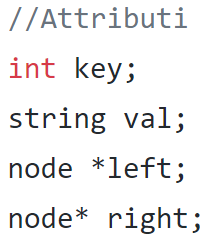
\includegraphics[width=3cm]{Attributi}
			    	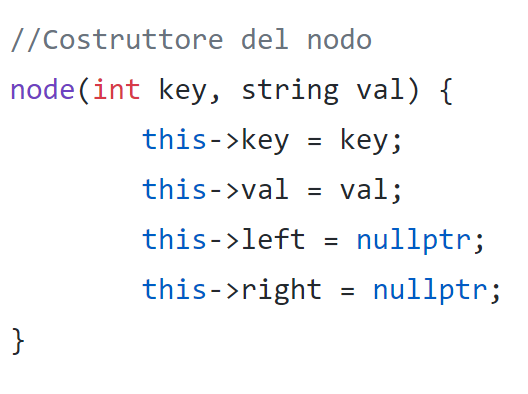
\includegraphics[width=4cm]{Creatore1}
			    \end{figure}
		    	Ogni nodo viene poi inizializzato grazie alla funzione \textbf{create} dove, una volta passati come parametri la chiave e il valore, mi crea il nodo. \\
		    	Successivamente possiamo trovare delle funzione di supporto che servono a rendere la struttura più versatile e facile da utilizzare:
		    	\begin{enumerate}
		    		\item \textbf{la funzione insert:} inserisce un nuovo nodo nell'albero di ricerca passatogli come argomento, assumendo che esso non sia già contenuto al suo interno;
		    		\item \textbf{la funzione find:} cerca all'interno dell'albero il nodo con chiave numerica k (passata come argomento) e restituisce (qualora esso esista) il valore di tipo stringa ad esso legato;
		    		\item \textbf{la funzione clear:} rimuove ricorsivamente tutti i nodi dall'albero, che diventerà quindi vuoto, liberando così la memoria;
		    		\item \textbf{la funzione min:} cerca il nodo con il valore minimo all'interno dell'albero;
		    		\item \textbf{la funzione remove:} elimina il nodo cercato sistemando poi i suoi figli, qualora essi esistano;
		    	\end{enumerate}
		 \newpage
		 	\subsection{Analisi e calcolo tempi}
	   	 \newpage
		\section{Alberi binari di ricerca di tipo AVL}
			\subsection{Introduzione}
			La seconda struttura dati che analizziamo è quella degli alberi creati da \textit{Adelson-Velsky and Landis (AVL tree)}.\\
			Oltre a soddisfare le proprietà di un albero di ricerca semplice, l'AVL ha una caratteristica in più: \textit{per ogni nodo x all'interno dell'albero, le altezze dei sotto-alberi di sinistra e di destra differiscono al massimo di 1.}\\
			Tale proprietà viene garantita \textit{eseguendo opportune rotazioni sui nodi sbilanciati}, partendo dal nodo sbilanciato più profondo e procedendo risalendo l'albero lungo il cammino di accesso a quel nodo.\\
			Per la loro rappresentazione è stata creata una classe che crea i singoli nodi, ognuno dei quali è composto da sei attributi:
			\begin{itemize}
				\item \textbf{key:} elemento che rappresenta la chiave numerica del nodo;
				\item \textbf{val:} elemento che rappresenta il valore del nodo sotto forma di stringa;
				\item \textbf{left, right e father:} rappresentano i figli del nodo, rispettivamente quello sinistro e destro, e il padre del nodo. Vengono inizializzati a \textit{NILL}.
				\item \textbf{height:} rappresenta l'altezza del nodo ed è inizializzato a 1;
			\end{itemize}
			Possiamo trovare una serie di funzioni che servono a rendere la struttura funzionante:
			\begin{enumerate}
				\item \textbf{la funzione get height:} ritorna l'altezza dell'albero;
				\item \textbf{la funzione destra e sinistra:} eseguono la rotazione dell'albero verso destra o sinistra;
				\item \textbf{la funzione valore di bilanciamento:} ritorna 0 se la root è null oppure sono perfettamente bilanciati, 1 se c'è più peso a sinistra oppure -1 se c'è più peso a destra;
				\item \textbf{tutte le funzioni viste precedentemente sui BST};
			\end{enumerate}
			
		\newpage
		
		\section{Alberi binari di ricerca di tipo Red-Black}
			\subsection{Introduzione}
			L'ultima struttura dati che analizzeremo è quella dei Red-Black Tree.\\
			Come prima cosa viene creata sia la tipologia di colore che un nodo può avere (ovvero \textit{nero} o \textit{rosso}), che la tipologia del nodo stesso (ovvero \textit{root}, \textit{left} o \textit{right}).\\
			\begin{figure}[ht]
				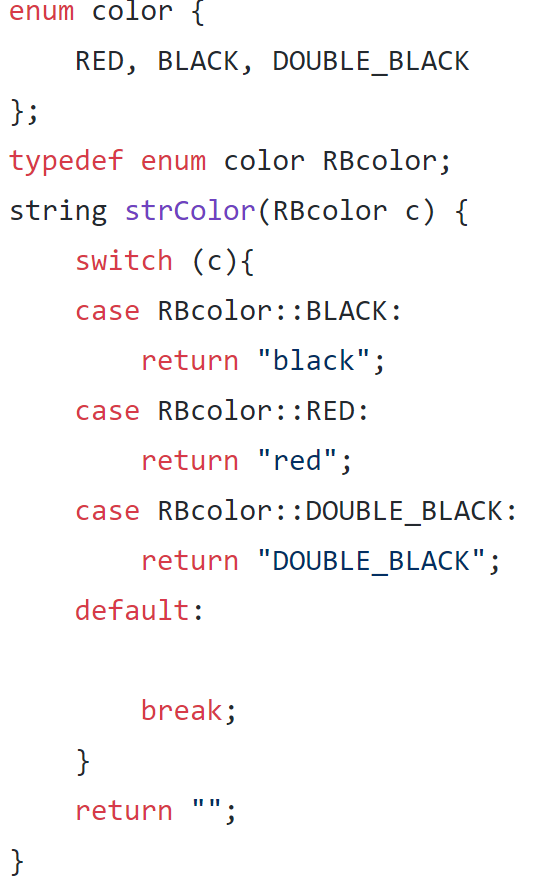
\includegraphics[width=3cm]{Enum}
			\end{figure}
			Proprio come per le altre due strutture, anche qui viene creata la stessa classe per la rappresentazione del nodo, con però l'aggiunta di attributi in più come \textit{il nodo padre} e \textit{il colore del nodo}.\\
			Troviamo inoltre la presenza degli stessi metodi dei BST con l'aggiunta di:
			\begin{itemize}
				\item \textbf{rotateR e rotateL:} rispettivamente ruotano a destra e sinistra l'albero grazie ad un perno passato come argomento e serve per ri-bilanciare l'albero;
				\item \textbf{getColor:} mi dice il colore del nodo passato come argomento;
				\item \textbf{uncle:} mi ritorna lo zio del nodo preso in considerazione;
				\item \textbf{grandfather:} mi ritorna lo zio del nodo preso in considerazione;
				\item \textbf{checkBST:} ritorna true qualora l'albero abbia tutti i puntatori giusti;
				\item \textbf{check:} ritorna true qualora l'RBT abbia tutti i puntatori giusti, colori giusti e black-height corretta;
			\end{itemize}
			
			\newpage
			\subsection{Analisi e calcolo tempi}
			\newpage
		\section{Algortimo per il calcolo dei tempi}
		Viene eseguita una stima dei tempi medi e \textbf{ammortizzati} per l'esecuzione di \textbf{n} operazioni, sia di inserimento che di ricerca, nelle tre strutture dati viste precedentemente. \\
		Viene scelto inizialmente un parametro \textbf{n} che corrisponde al numero di operazioni che vogliamo che vengano fatte su un albero inizialmente vuoto. Le operazioni che vengono eseguite sono:
		\begin{enumerate}
			\item \textbf{generazione in modo pseudo-casuale del valore k};
			\item \textbf{ricerca di un nodo con chiave k};
			\item \textbf{qualora esso non esista, si crea un nuovo nodo con chiave k e lo si inserisce all'interno della struttura};
			\item \textbf{gestione della memoria:} ad ogni iterazione la memoria viene cancellata grazie ai metodi \textit{clear} presenti dentro al codice degli alberi.
		\end{enumerate}
		Infine abbiamo che il tempo ammortizzato di tutte le operazione eseguite è il risultato dato da il \textit{tempo totale impiegato per l'esecuzione delle operazioni diviso il parametro n}.\\
		Abbiamo ottenuto quindi un tempo ammortizzato che ha un errore relativo che non supera mai 
		\textbf{l'1\%}
	
\end{document}